\documentclass{article}

% Packages
\usepackage{indentfirst}
\usepackage{fullpage}
\usepackage{graphicx}
\usepackage{hyperref}
\usepackage{float}
\usepackage{listings}
\usepackage{mdframed}


\title{Algorithms and Optimization Techniques for Solving TSP}
\author{Raiyan Mahbub \\ mahbu006@umn.edu \\ University of Minnesota}
\date{\today}

\begin{document}
\maketitle

\begin{abstract}
    
The traveling salesman problem (TSP) is one of the most extensively studied optimization problems in the computer science and computational mathematics field given that there is yet an optimal solution for it to be discovered. This algorithmic problem asks that if we are given a list of n places and the distances between each pair, what is the shortest possible route that visits each city exactly once and returns to its initial starting point. In this paper, we will be conducting a comparative study to test and evaluate the performance of three algorithms: Simulated Annealing, Ant Colony Optimization, and Genetic Algorithm. With the traveling salesman problem classifying under NP-hard computational complexity, we will be examining the runtime as well as the shortest distance computed by each of these algorithms by setting up analogous environments of n cities. \\
\end{abstract}


\section{Introduction}
One of the most critical tasks of engineers and scientists around the world is to perpetually pursue the concept of optimization. Whether that being to design more efficient and effective systems, or generate cost-effective methods to improve scalability, scholars are constantly looking for ways to achieve optimality by devising and developing techniques to improve the operations of systems in various fields. This includes the conventional traveling salesman problem (TSP) which is an NP-hard problem in combinatorial optimization vastly studied in algorithms and operational research. This well known algorithmic problem asks: given a list of n cities and the distances between each pair of cities, what is the most efficient (i.e. shortest possible route) that visits each city exactly once and returns to its initial starting point. The pure simplicity of this problem is quite deceptive as TSP is one of the most extensively studied optimization problems in the computer science and computational mathematics field. \\
\par To emphasize the intricacy of the TSP, let us suppose we were visiting the minuscule country of Maldives. Suppose we wanted to determine the most optimal path to travel to every city in Maldives (they have approximately ~30) and frame it as a TSP. To compute all of the paths between them, the possible combinations of visiting all sequences of cities is 30! or $2.65 \times 10^{32}$. To put this unfathomable number into perspective, if we were to try every possible combination and test $10,000$ sequences \textit{per second}, it would take modern computers over 8 million years to observe the solution. The intriguing traveling salesman problem was first introduced in 1930, and a wide variety of applications stemmed from it. It gradually became a benchmark for countless other optimization problems and started appearing as real life applications such as: arranging bus routes to pick up passengers, scheduling a machine to drill holes in a circuit board, radiation hybrid maps in genome sequencing, etc. An optimal solution for TSP has yet to be discovered, however some intricate non-optimal solutions have approached optimality with a fast runtime.


\section{Literature Review}
\subsection{Overview}
In this literature review, we will explore common algorithms that have been used to solve TSP from scientific journals and articles and analyze the distinct approaches and their corresponding metrics. While being a classical combinatorial optimatization problem, TSP has an vast search space and cannot be solved in polynomial time, or NP-hard. In particular, we will examine a genetic algorithm with modified cycle crossover operator, the nearest neighbor algorithm, and the traditional greedy algorithm, and several more approaches for solving TSP. We will also be investigating into what specific qualities make TSP to become an NP-hard problem and briefly explore computational complexity theory. 
  
\subsection{Genetic Algorithm}
The traveling salesman problem is one of the most fundamental problems in the field of computer science and optimization in modern research. According to Sangwan in \cite{sangwan},there are countless applications of TSP such as: printed circuit board drilling, manufacturing of microchips, packet routing in mobile communications, vehicle routing, etc. Many different algorithms and heuristic techniques have been utilized to determine an efficient solution to TSP, but as the number of nodes increase, the computation becomes quite complex. For instance in \cite{hussain}, Hussain, et al examine the genetic algorithms, or GAs, which is essentially a search heuristic derived from the concept of Darwinism and the theory of natural evolution. This algorithm fundamentally reflects the process of survival of the fittest, where the best individuals of each generation are selected for reproduction. Thus, the next generation should be healthier and fitter than its prior one. The authors propose in \cite{hussain} a new crossover operator for the traveling salesman problem to minimize the distance traveled. They argue that the most natural way to represent a legal tour is by using an approach connected with path representation. After running various forms of tests with different selection criteria, crossover and mutation operators, they were able to determine that the CX2 operator performs significantly better than PMX and OX. \\


\subsection{Nearest Neighbor and Greedy Algorithms}
Regarding the study done by Kizilates and Nuriyeva in \cite{kizilates}, the authors researched a modified version of the nearest neighbor algorithm for TSP. This algorithm follows the steps outlined: first a random city is selected, then it finds the nearest unvisited city and travels there. It then checks if there are any unvisited cities left and if goes there. If not, it returns back to the original city where it started from. The modification made in this study was that they utilized greedy algorithms from different endpoints as well as the nearest neighbor. After running multiple computational experiments in \cite{kizilates}, Kizilates and Nuriyeva demonstrated that this hybrid algorithm is indeed efficient on well-known library problems. The last article done by Ejim \cite{ejim}, is on how greedy algorithms themselves can be applied to TSP. A greedy algorithm essentially makes the locally optimal selection at each stage of the algorithm hoping to find the optimum. While this algorithm may not always be the most effective nor the most efficient, it could in a reasonable time possibly yield locally optimal solutions which could approximate the globally optimal solution. After running a profile on their tests, they found that the time complexity was exponential and the time needed to run the algorithm increased significantly as the problem size was increased. \\


\subsection{Optimization Methods}
We can also observe there are different optimization methods can be applied to the generalized traveling salesman problem. For instance in \cite{fang}, Fang, et al. illustrates the particle swarm optimization (PSO) with simulated annealing in the 6th WSEAS International Conference on Artificial Intelligence. They proposed an advanced PSO algorithm that does not easily become trapped in a local minimum with the addition of simulated annealing. The SA method is essentially utilized to slow down the degeneration of the PSO swarm as well as increasing the swarm's diversity. Based on their comparative experiments, PSO-SA was distinctly superior compared to the conventional genetic algorithm, basic simulated annealing, and the adaptive cross approximation algorithm to solve the TSP. Another optimization used for solving the generalized TSP is the ant colony method presented by Yang, et al. in \cite{yang}. They primarily focused on a variation of the euclidean TSP and they were searching for techniques to avoid locking into a local minimum similar to \cite{fang}. They introduced a mutation process and local searching algorithm derived from observing real ants who are capable of finding the shortest path from a food source to their nest without the need for visual cues through probability techniques. \\

\subsection{Computational Complexity Theory}
Looking into what qualities make a problem NP-hard, Paschos effectively conveys it in \cite{Paschos} as that no polynomial algorithm can really be devised for an optimal solving of any NP-hard problems. However, this intricacy robustly motivates both practitioners and researchers to attempts to solve these problems heuristically. This inherently creates a trade-off between computational time and the quality of the optimal solution. This polynomial approximation theory deals with solving a given NP-hard problems in polynomial time by computing feasible solutions as close to optimal as possible under some predefined criterion. Examining from a broader context, we have to look at computational complexity theory which is a central field of the theoretical foundations of the computer science field. Goldreich in \cite{Goldreich} defines this theory with the study of the intrinsic complexity of computational tasks. More specifically, their studies refer to the computational resources that are required to solve a computational class of tasks such as the traveling salesman problem. The theory additionally looks at what tasks can be achieved with either limited time and limited computational resources. The traveling salesman problem is an exemplary practical application of the computational complexity theory as the algorithmic problem is difficult to optimize when the input becomes arbitrarily large.


\section{Approach}
\subsection{Simulated Annealing}
Simulated Annealing (SA) algorithm is a stochastic technique that can be useful for determining the global optimum. The term ”annealing” stems from a thermodynamic analogy, more specifically the way that metals cool; SA uses its objective function of an optimization problem rather than the energy of a material. This materials science parallelism additionally involves the introduction of noise to avoid search failure due to a local minima or plateau. To enhance or improve the probabilistic odds of determining the global optimum rather than a sub-optimal local one, a stochastic element to the algorithm is integrated by simulating Brownian thermal motion. Some forms of this simulated annealing consist of the injection of randomized numbers with variety of distributions or the averaging effect of mini-batching which is essentially splitting a batch into segments and performing a slight network parameter adjustment after each iteration. \\
\par When applying SA to the TSP, we maintain the temperature to be variable to simulate the said heating process. While initially leaving it high, we gradually cool it off as the algorithm continues to iterate. The high temperature will correspond to an increased frequency to which we accept proposed solutions, or shortest paths to cities in this case, and it will incline towards accepting solutions that are actually worse than our current ones. This freedom allows the SA algorithm avoid getting stuck in any local optima early on in the algorithm. However, as said before the temperature is systematically reduced and the chances of accepting worse solutions decrease as well. Thus, SA eventually maintains focus on a search space that is hopefully around an optimal solution. This measured cooling process is what will make the application to TSP so effective as we are dealing with a vast search space with an abundance of local optima. 

\subsection{Ant Colony Algorithm Optimization}
The Ant Colony optimization is one of the more popularized meta-heuristics utilized in combinatorial optimization in which the algorithm seeks an optimal solution in a discrete search space. The Ant Colony Optimization (ACO) is essentially derived on computations from real ant colonies and how they operate in nature. An ant's primary behavior is fundamentally dominated by the goal of the survival of the colony rather than their own interests. ACO is more specifically based on the keen seeking behavior of ants and how they are able to quickly find shortest paths between food sources and their temporary homes. When they are initially searching for a food source, they discover the said aforementioned area through a stochastic process. While trotting along, each and every ant leaves behind a chemical pheromone trail in the ground which can be sensed by other ants. The following diagram conveys the process of the ant colonies leaving behind the scent, and effectively picking it back up after iterations:
\begin{figure} [H]
  \centering
  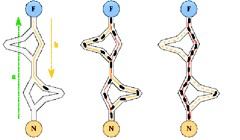
\includegraphics[width=10cm, height=4cm]{ACA_Diagram.jpg}
      \caption{Ants use pheromone as indirect communication to build best tour \cite{Alhanjouri}}
\end{figure}
The next time the colony of ants path towards their food source, they probabilistically select paths with strong pheromone concentrations. They strengthen these concentrations if the food is perhaps of more quality or more plentiful as well. These indirect chemical substances have shown that they enable these ant colonies to locate the shortest path between their homes and food. We will be using this exact approach for our generalized n-cities traveling salesman problem by exploiting the exploratory and randomness nature of the algorithm along with increasing the attractiveness of the pheromones to the ants.


\subsection{Genetic Algorithm}
Genetic algorithms, or GAs, are essentially a search heuristic algorithm derived from the concept of Darwinism and the theory of natural evolution and development. They are search methods based on the principles of symbiosis, fitness test, mutation, meiosis, breeding, extermination of insufficiency, and recursion. The GA initially begins with a wide set of solutions which are denoted by chromosomes called the population. The solutions from the single population are kept and are used to breed and form a new population. Motivated by optimism, the genetic algorithm hopes to retrieve a new generation that will be better and more optimal than the previous generation. The solutions that are selected by the algorithm are denoted as the offspring undergo the fitness evaluation function. They are judged accordingly by their fitness attributes, and the more suitable the offspring, the higher probabilistic chance they will be the parents to form the next generation and replicate. The pseudocode outlined by Mukhairez, et al. in \cite{Mukhairez} for the genetic algorithm is as follows: 

\begin{enumerate}
	\item Generate a randomized population of n chromosomes
	\item Evaluate the fitness function for each chromosome x in the current population
	\item Form a new population with the following until complete:
    \begin{enumerate}
    	\item Select two parent chromosomes from current population according to fitness evaluation
        \item Perform a probabilistic cross-over with the parents to form offspring
        \item Mutate new offspring at each locus, or position in the chromosome
        \item Place new offspring into the newly generated population
    \end{enumerate}
    \item Use new population for an extended run of the genetic algorithm
    \item If end condition is satisfied, terminate procedure and return best solution in current population
    \item Iterate beginning from step 2
\end{enumerate}


\section{Experimental Design and Results}
\subsection{Experiment Implementation}
To run these experiments for the SA, ACO, and GA algorithms, we utilized two open-source libraries and repositories from GitHub. The first one being scikit-opt which is a powerful Python library and module built specifically for heuristic algorithms from \cite{guofei} to which we deployed the SA and ACO algorithms. For GA, we used the TSP-GA repository from \cite{lccasagrande} which used cities in Brazil for its computation. We proceeded to run several executions of all three of these algorithms through Python from these APIs using both n = 15 and n = 50 cities. This was implemented through a randomly generated function on a coordinate plane along with a procedure that computed the shortest distance the algorithms were able to find as follows: \\

\begin{mdframed}
\begin{lstlisting}[language=Python]
num_cities = 15   # number of cities
points_coordinate = numpy.random.rand(num_cities, 2) # generate points
distance_matrix = spatial.distance.cdist(points_coordinate, 
                                         points_coordinate, 
                                         metric='euclidean')
                                         
def cal_total_distance(routine):
    # the objective function. input routine, return total distance.
    num_cities, = routine.shape
    return sum([distance_matrix[routine[i % num_cities], 
           routine[(i + 1) % num_cities]] for i in range(num_cities)]) 
\end{lstlisting}
\end{mdframed}

All of the simulations were completed on a i5-8265U processor clocked at 1.60GHz, 1800 MHz with 8 GB of RAM. For the simulated annealing algorithm, we used the parameters of T\_max = 100 (\textit{initial temperature}), T\_min = 1 (\textit{end temperature}), L = 10 * num\_cities (\textit{iterations under temperature}). For the ant colony optimization algorithm, we tuned the parameters to size\_population = 50, max\_iterations = 200, alpha = 1 (\textit{control parameter}), beta = 2 (\textit{control parameter}), rho = 0.1 (\textit{pheromone persistence coefficient}). Regarding the genetic algorithm, we focused on utilizing a contrasting data set of 15 cities in Brazil as this repository was a bit more trivial than the powerful scikit-opt engine for the other algorithms. We the parameters for GA to: population\_size = 500, tournament\_size = 50, mutation\_rate = 0.02, next\_gen = 20. For each experiment on these algorithms, we noted the execution time, number of iterations, quality of results, and captured the visualization of how the shortest paths were formed between the cities. 


\subsection{Results}
\subsubsection{Simulated Annealing}
\begin{table}[H]
\centering
\begin{tabular}{|c|c|c|c|l|}
\hline
\textit{}      & Trial 1 & Trial 2 & Trial 3 & Average \\ \hline
Total Distance & 4.3844  & 3.3165  & 4.7013  & 4.1341  \\ \hline
Time (ms)      & 0.1102  & 0.1299  & 0.1165  & 0.1738  \\ \hline
\end{tabular}
\caption{Simulated Annealing on TSP (15 cities)}
\label{tab:my-table}
\end{table}

\begin{figure} [H]
    \centering
    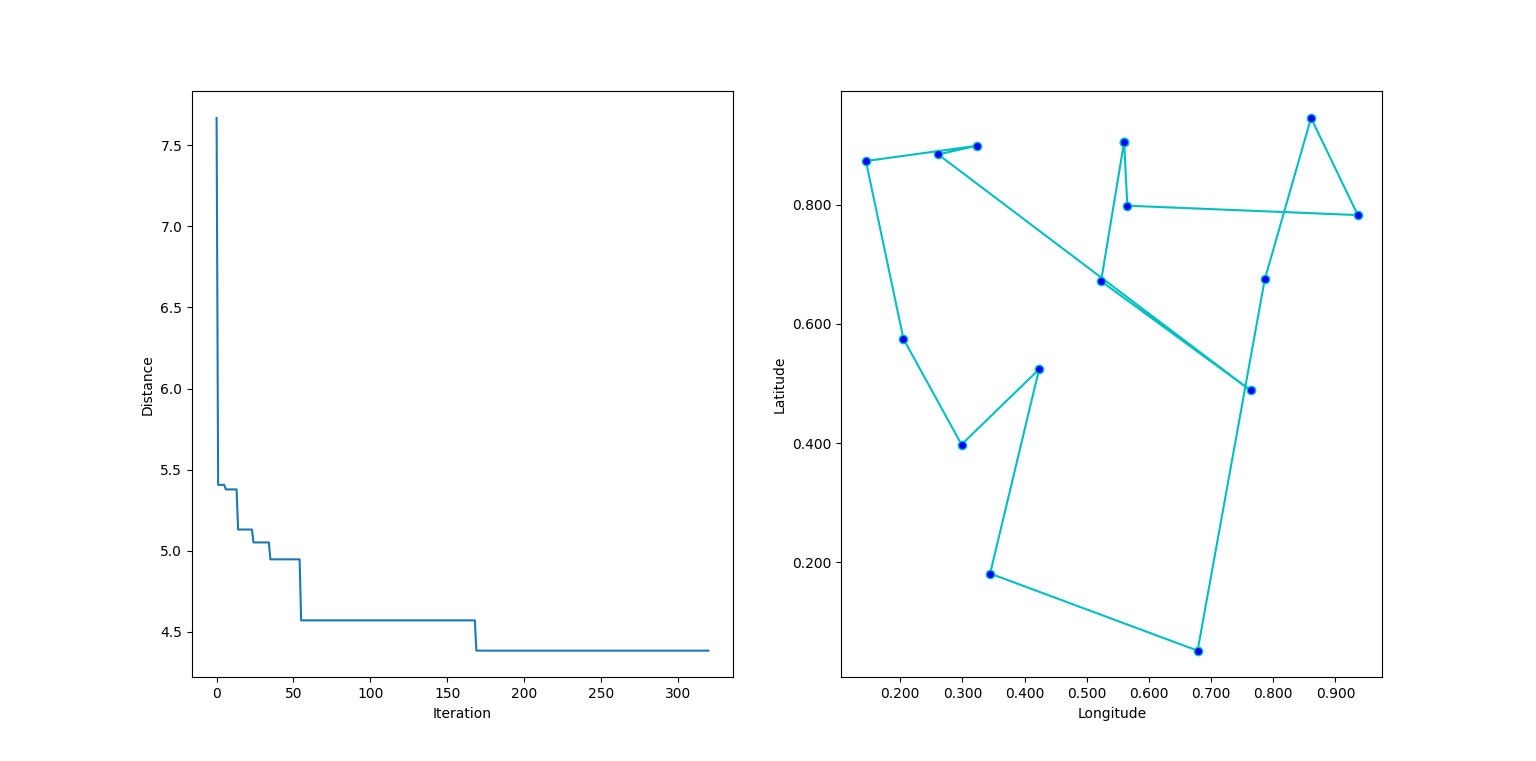
\includegraphics[width=0.6\textwidth]{SA_15cities_Trial1.png}\hfill
    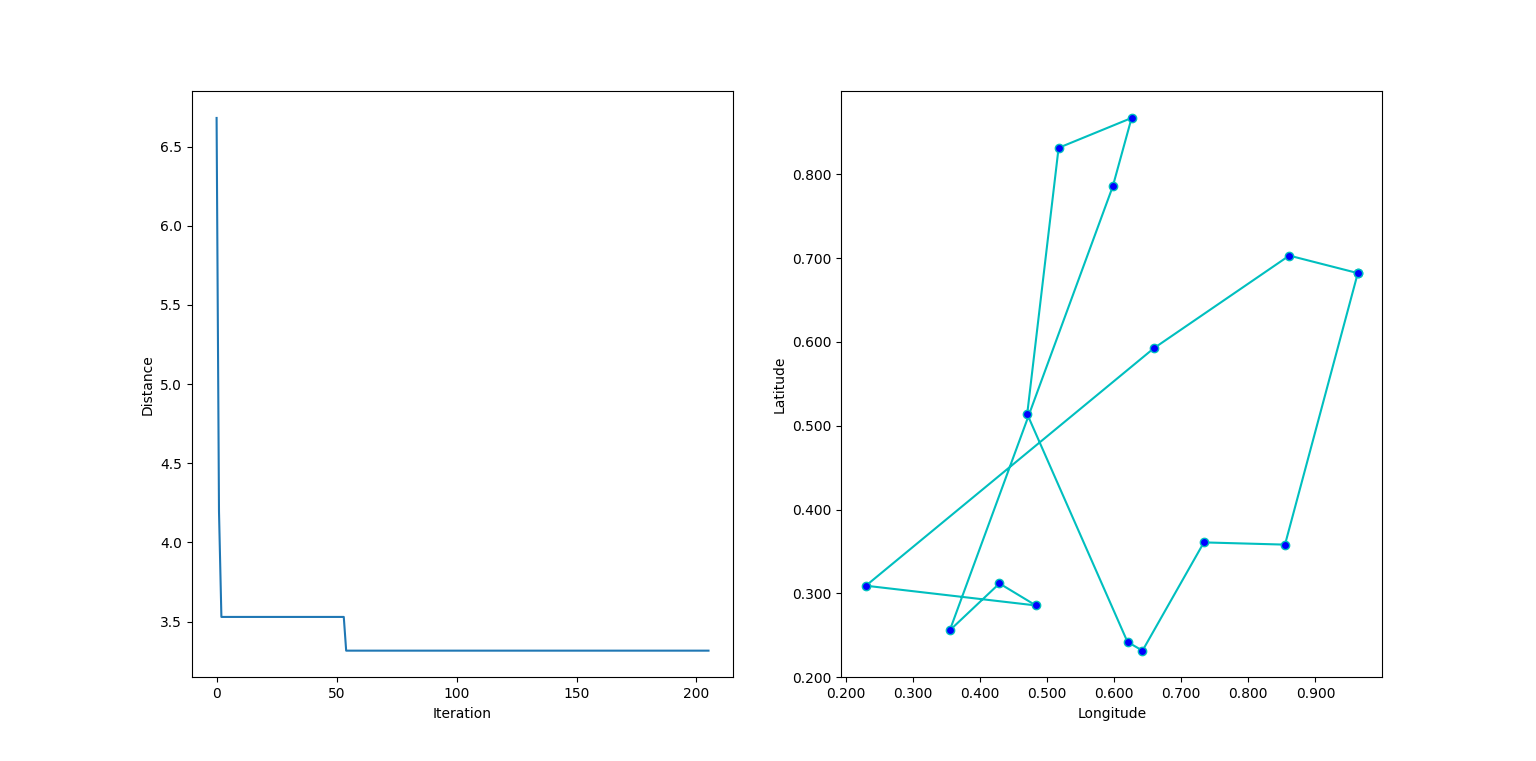
\includegraphics[width=0.6\textwidth]{SA_15cities_Trial2.png}\hfill
    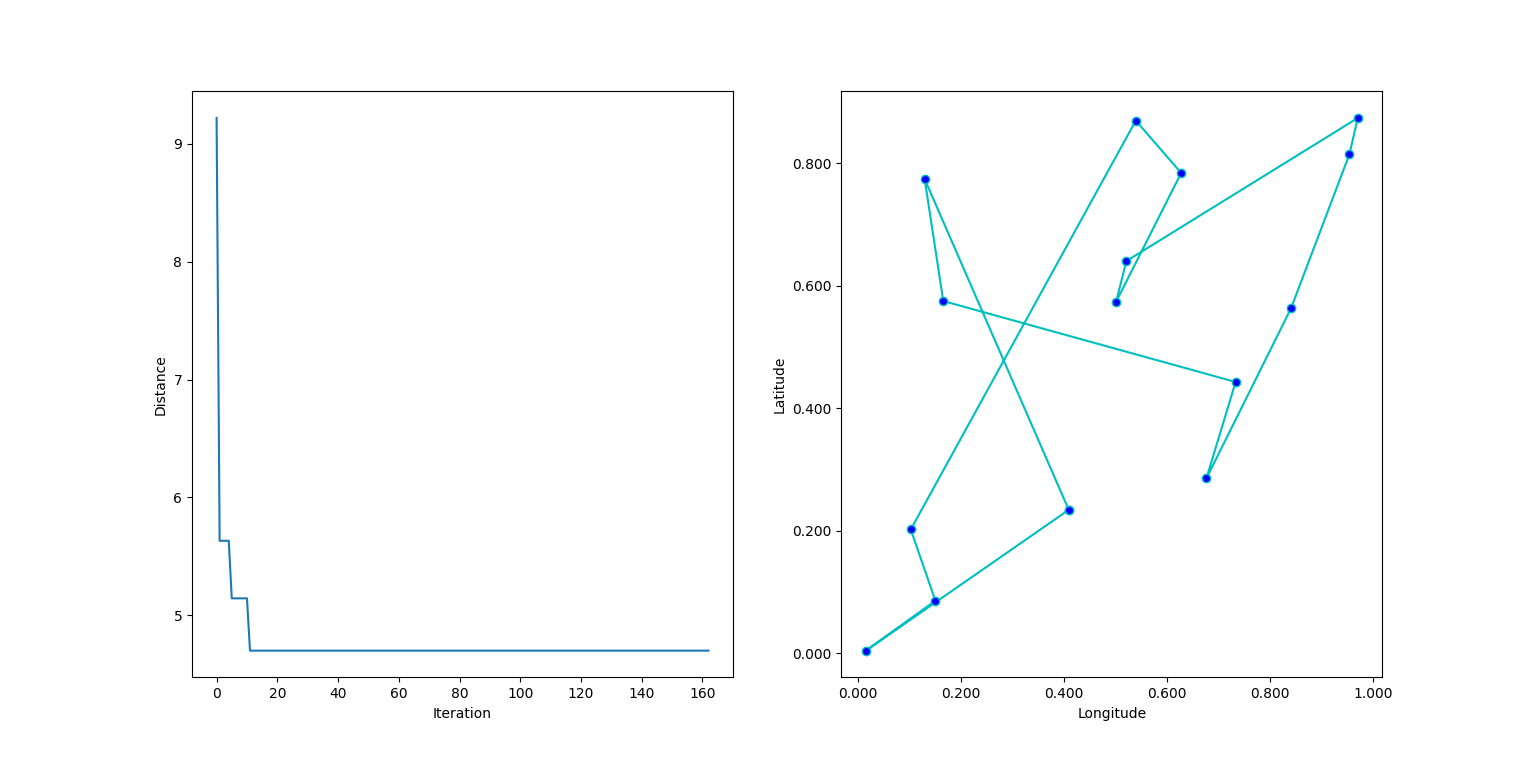
\includegraphics[width=0.6\textwidth]{SA_15cities_Trial3.png}
    \caption{Visual of Iterations and Shortest Path by SA (15 cities)}
    \label{fig:my_label}
\end{figure}

\begin{table}[H]
\centering
\begin{tabular}{|c|c|c|c|l|}
\hline
\textit{}      & Trial 1 & Trial 2 & Trial 3 & Average \\ \hline
Total Distance & 19.7649 & 21.7478 & 18.8821 & 20.1316 \\ \hline
Time (ms)      & 0.1634  & 0.1599  & 0.1582  & 0.1606  \\ \hline
\end{tabular}
\caption{Simulated Annealing on TSP (50 cities)}
\label{tab:my-table}
\end{table}

\begin{figure} [H]
    \centering
    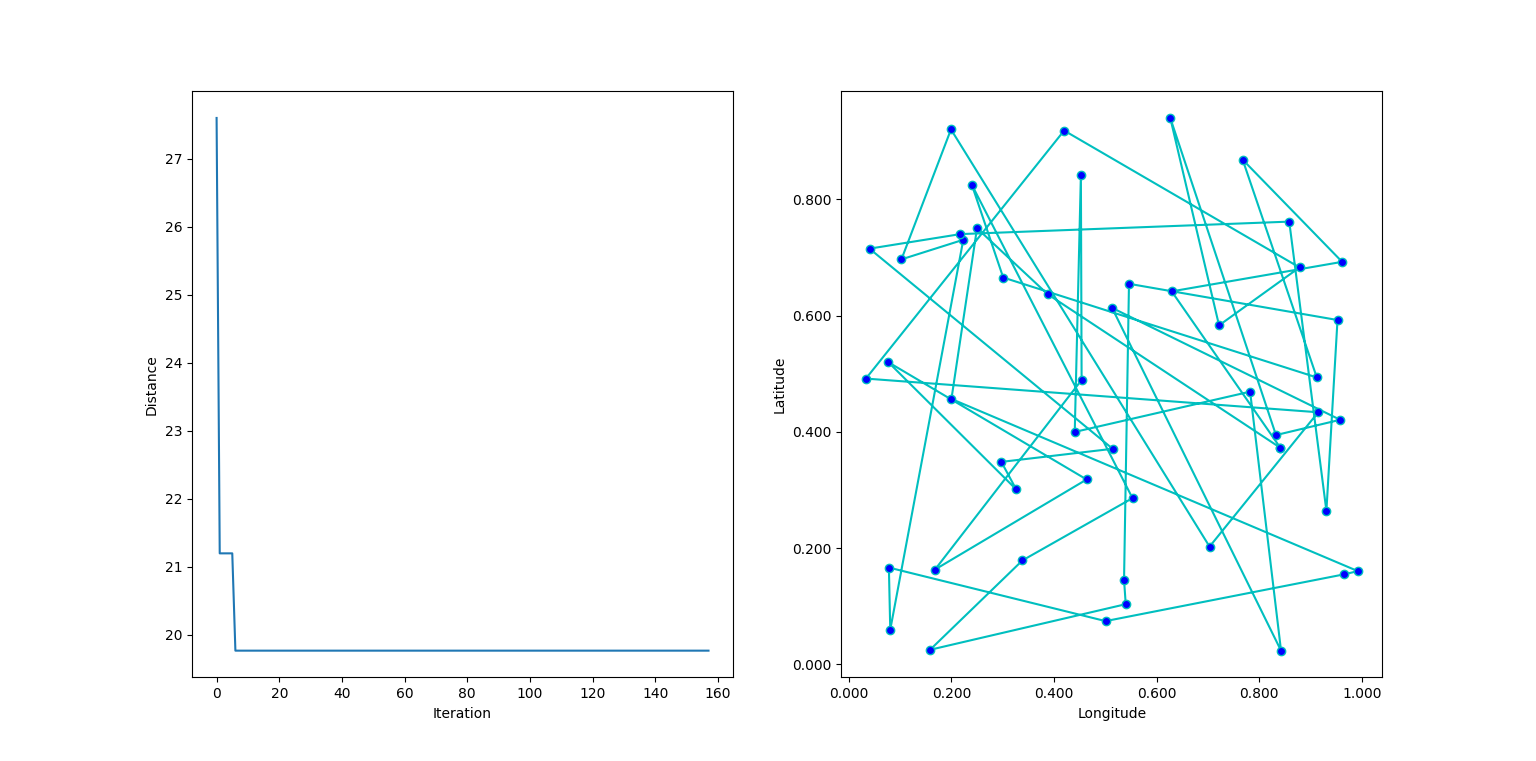
\includegraphics[width=0.6\textwidth]{SA_50cities_Trial1.png}\hfill
    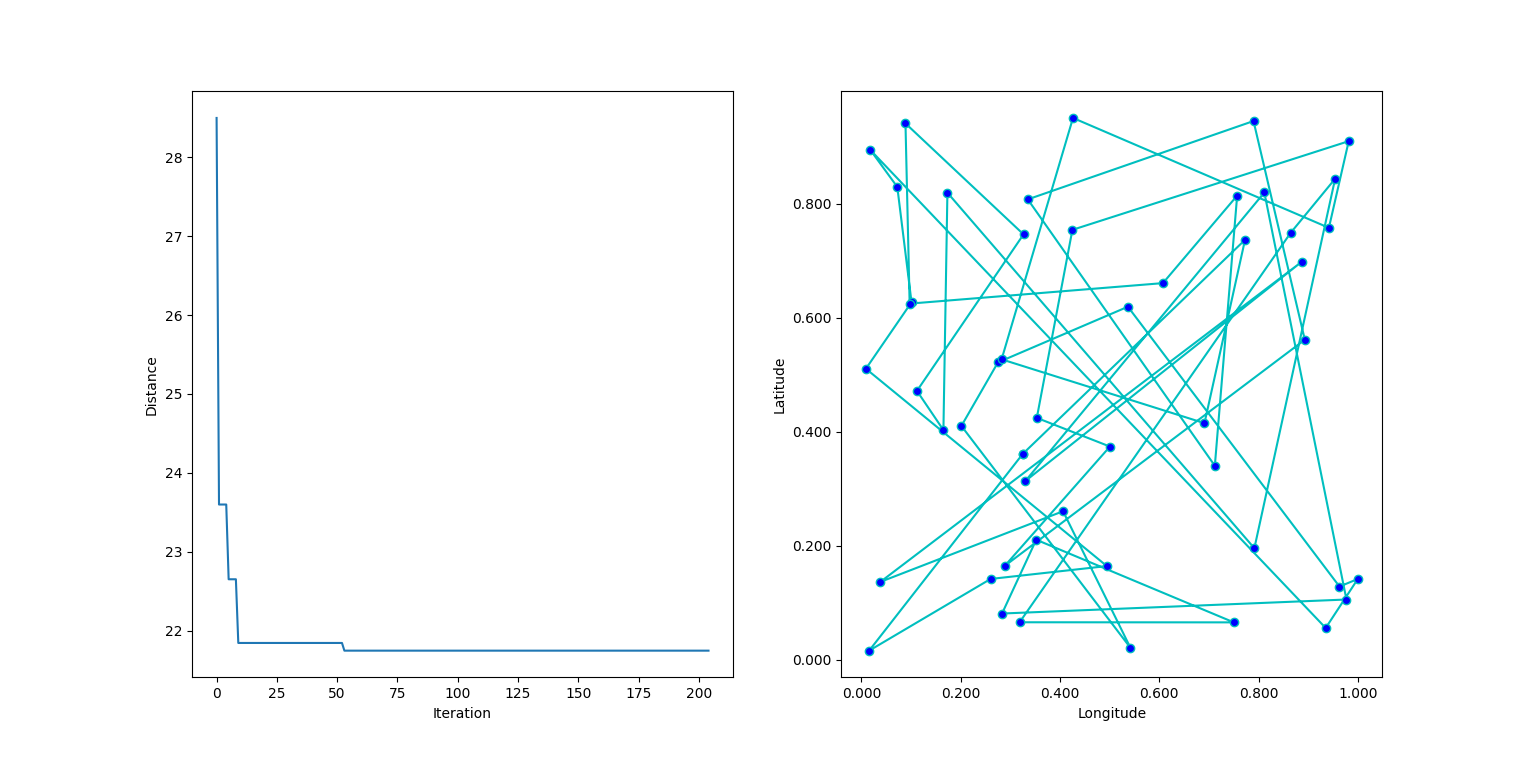
\includegraphics[width=0.6\textwidth]{SA_50cities_Trial2.png}\hfill
    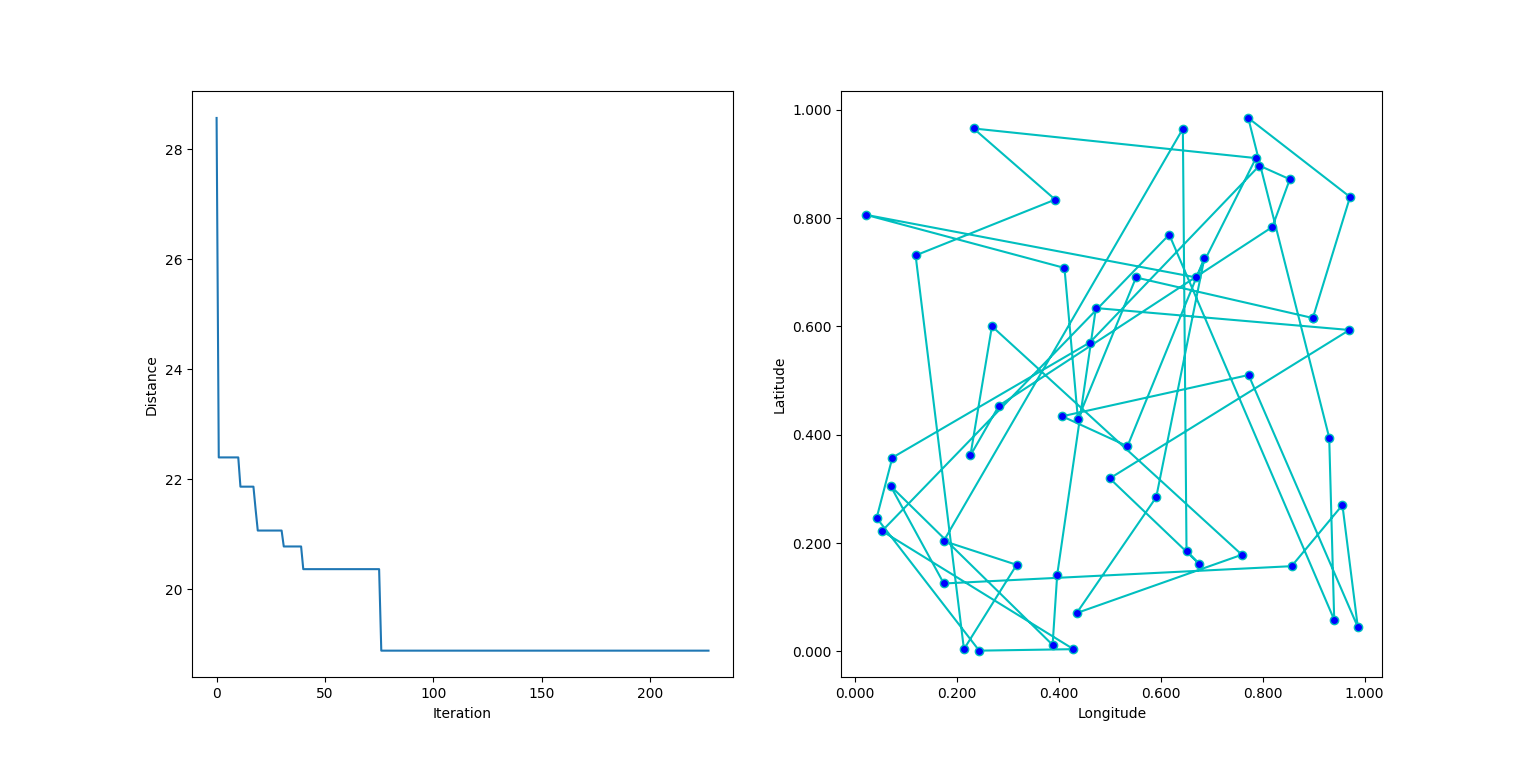
\includegraphics[width=0.6\textwidth]{SA_50cities_Trial3.png}
    \caption{Visual of Iterations and Shortest Path by SA (50 cities)}
    \label{fig:my_label}
\end{figure}


\subsubsection{Ant Colony Optimization}
\begin{table}[H]
\centering
\begin{tabular}{|c|c|c|c|l|}
\hline
\textit{}      & Trial 1 & Trial 2 & Trial 3 & Average \\ \hline
Total Distance & 4.1019  & 3.7308  & 3.8979  & 3.9102  \\ \hline
Time (ms)      & 2.0989  & 1.3563  & 1.7627  & 1.7393  \\ \hline
\end{tabular}
\caption{Ant Colony Optimization on TSP (15 cities)}
\label{tab:my-table}
\end{table}

\begin{figure} [H]
    \centering
    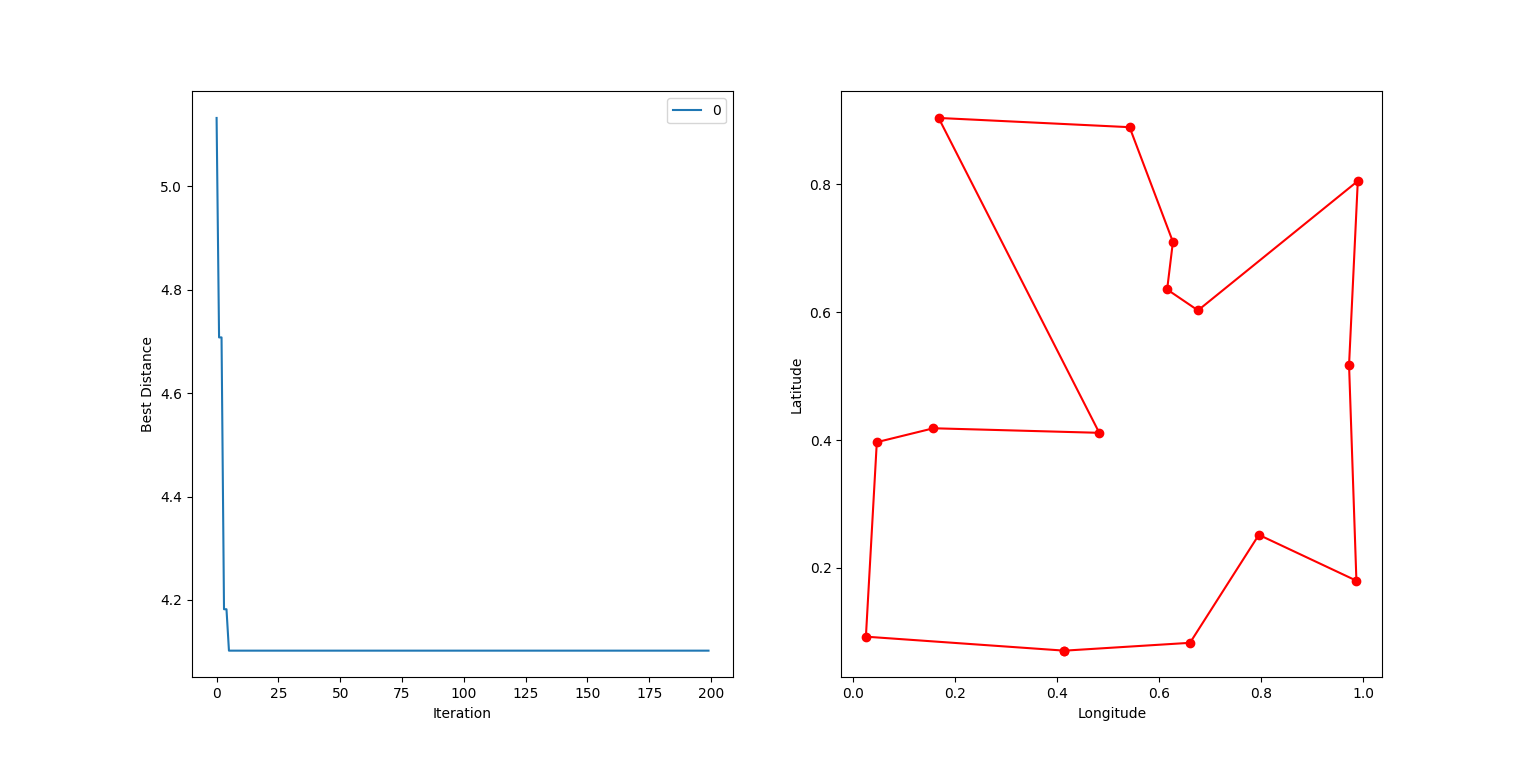
\includegraphics[width=0.6\textwidth]{ACA_15cities_Trial1.png}\hfill
    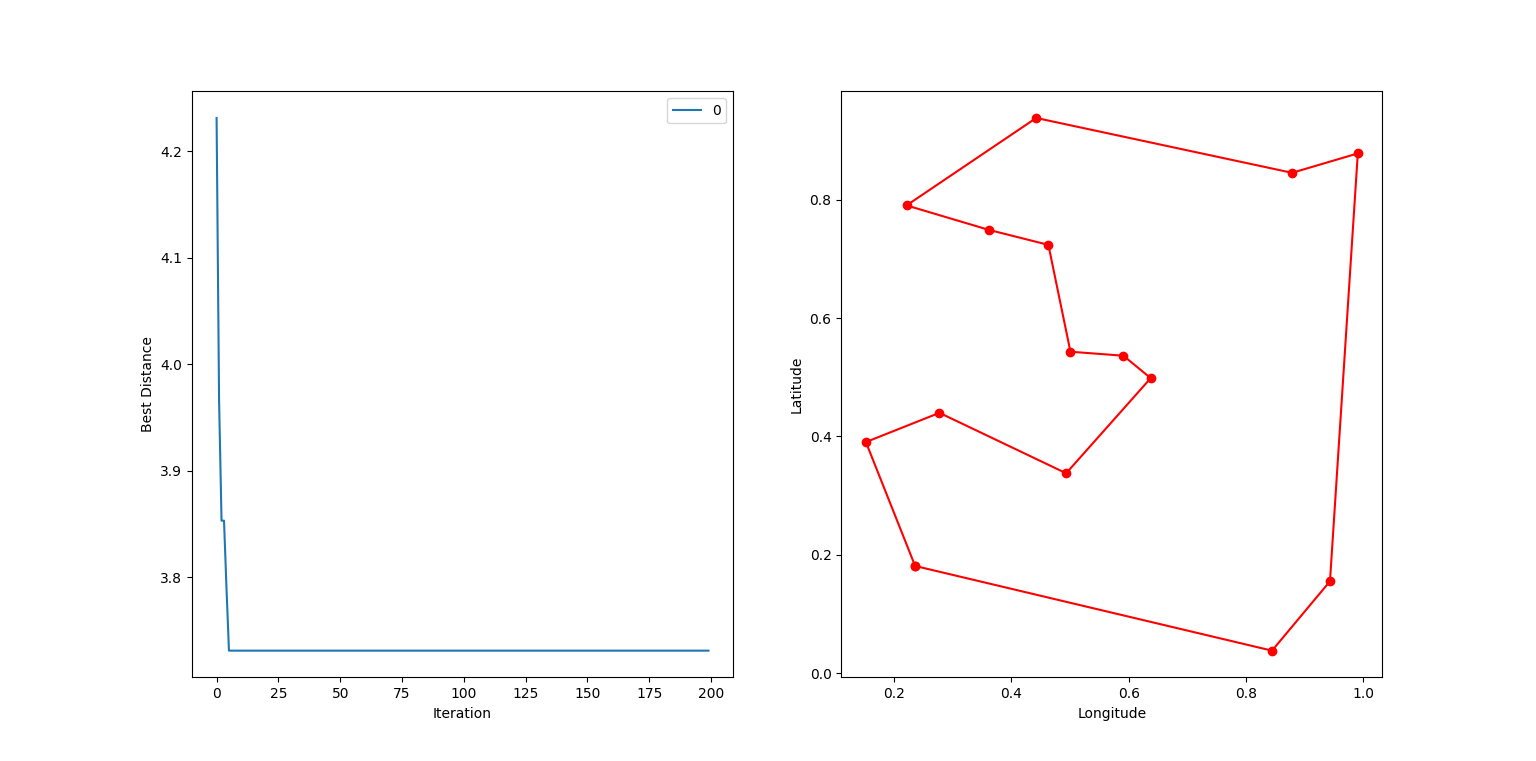
\includegraphics[width=0.6\textwidth]{ACA_15cities_Trial2.png}\hfill
    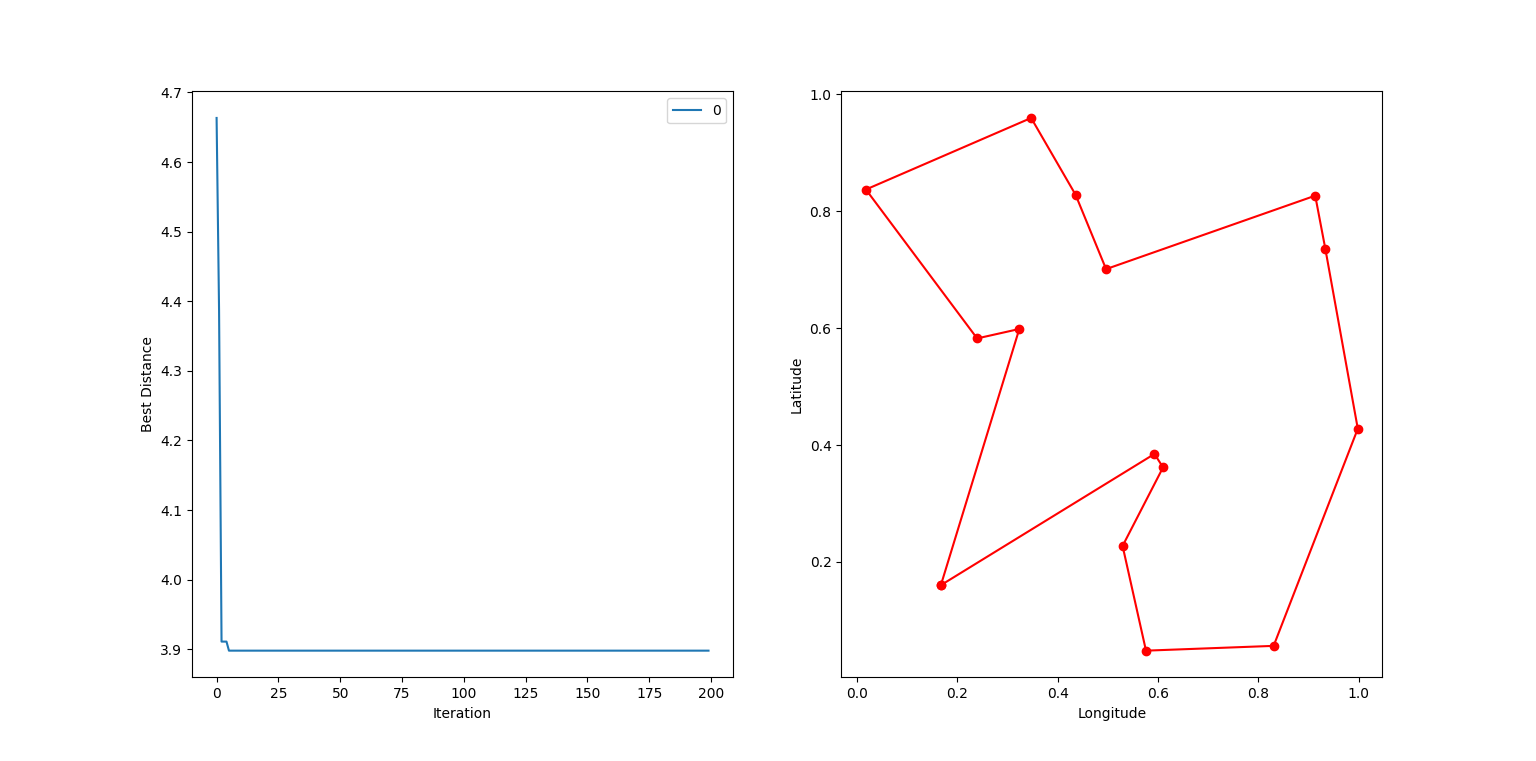
\includegraphics[width=0.6\textwidth]{ACA_15cities_Trial3.png}
    \caption{Visual of Iterations and Shortest Path by ACO (15 cities)}
    \label{fig:my_label}
\end{figure}

\begin{table}[H]
\centering
\begin{tabular}{|c|c|c|c|l|}
\hline
\textit{}      & Trial 1 & Trial 2 & Trial 3 & Average \\ \hline
Total Distance & 5.8374  & 6.0392  & 6.1615  & 6.0127  \\ \hline
Time (ms)      & 2.2064  & 2.7092  & 2.5034  & 2.2630  \\ \hline
\end{tabular}
\caption{Ant Colony Optimization on TSP (50 cities)}
\label{tab:my-table}
\end{table}

\begin{figure} [H]
    \centering
    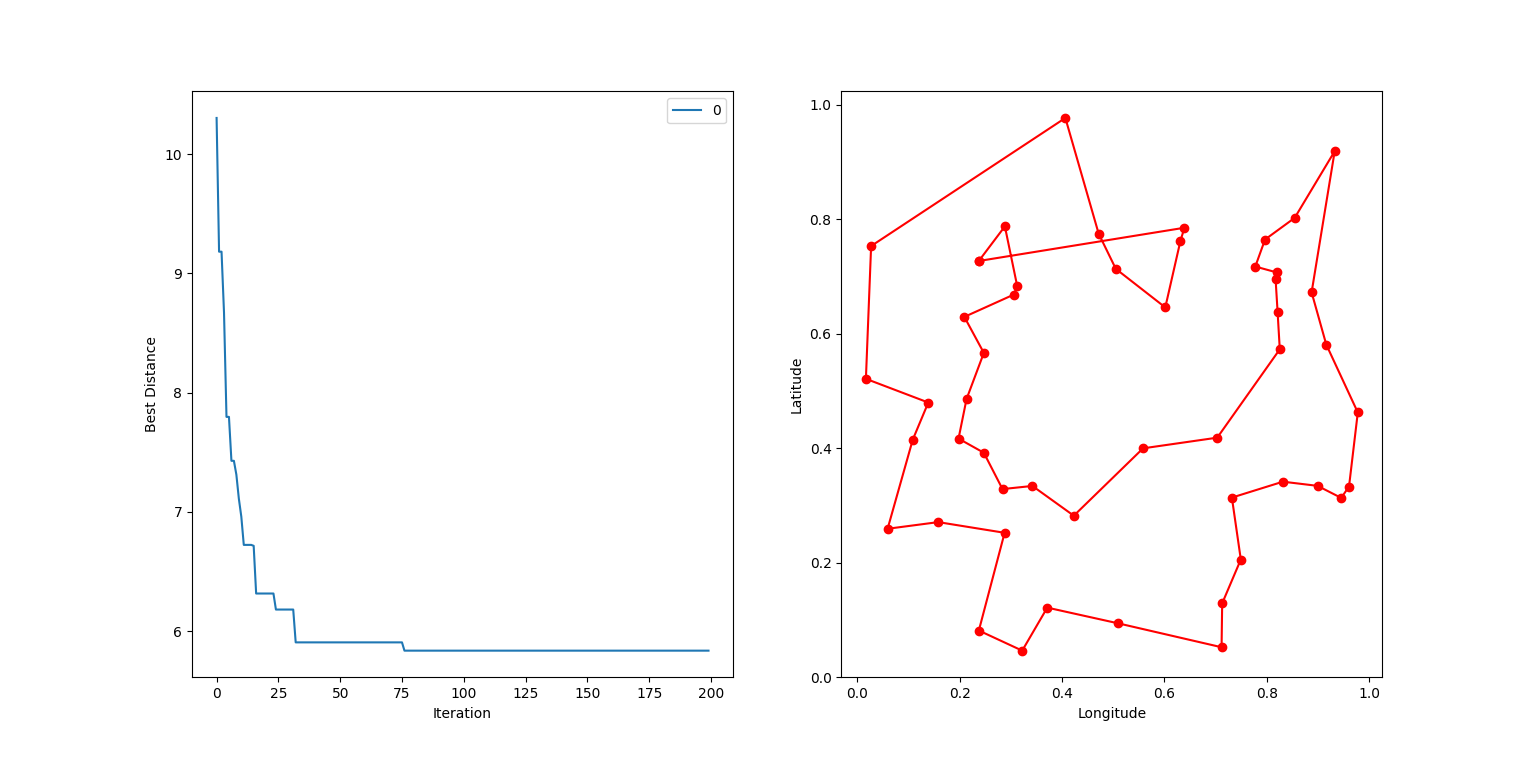
\includegraphics[width=0.6\textwidth]{ACA_50cities_Trial1.png}\hfill
    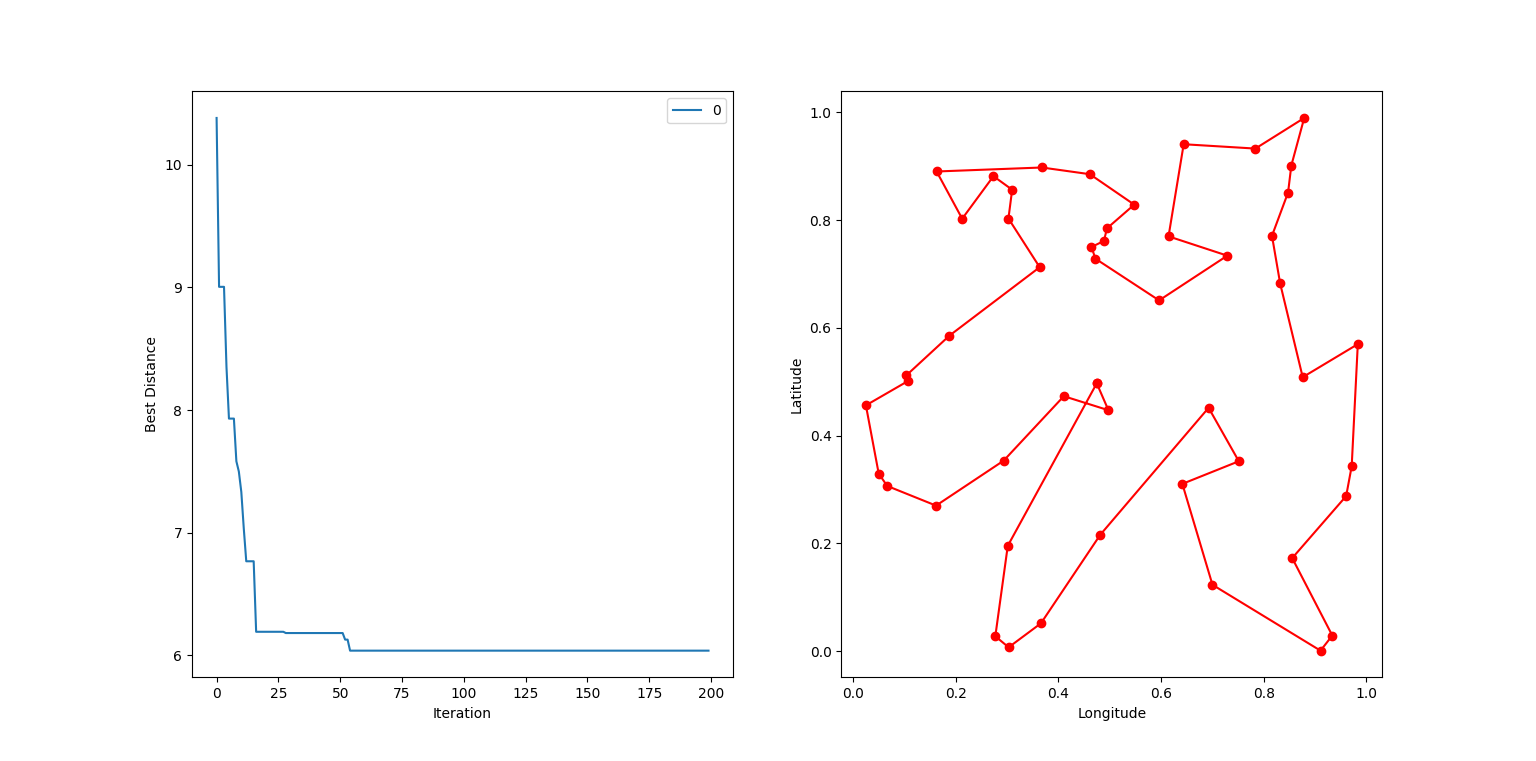
\includegraphics[width=0.6\textwidth]{ACA_50cities_Trial2.png}\hfill
    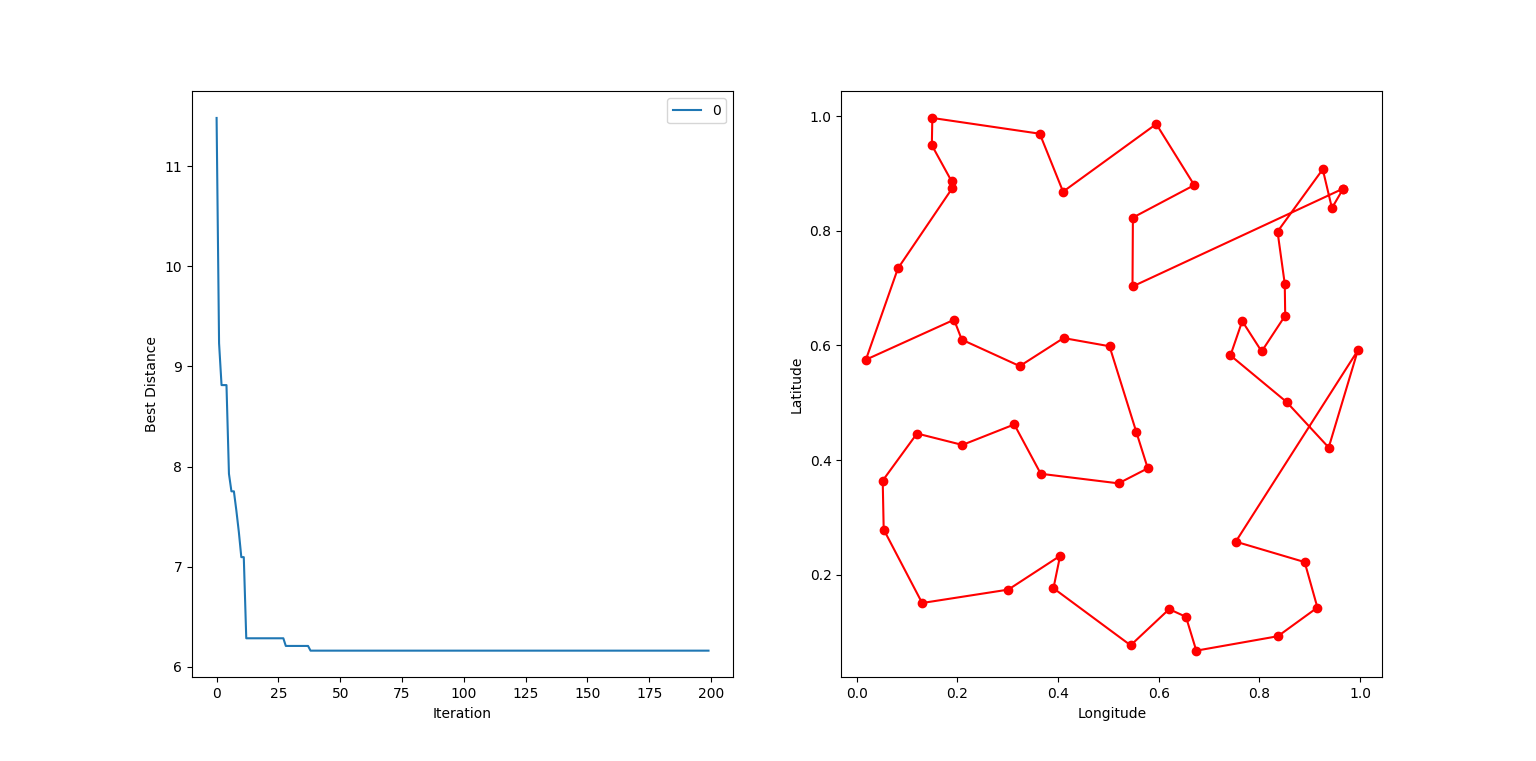
\includegraphics[width=0.6\textwidth]{ACA_50cities_Trial3.png}
    \caption{Visual of Iterations and Shortest Path by ACO (50 cities)}
    \label{fig:my_label}
\end{figure}

\subsubsection{Genetic Algorithm}

\begin{table}[H]
\centering
\begin{tabular}{|c|c|c|c|c|c|c|}
\hline
\textit{}           & Trial 1 & Trial 2 & Trial 3 & Trial 4 & Trial 5 & Average \\ \hline
\# of Generations   & 24      & 29      & 28      & 29      & 27      & 27.4    \\ \hline
Total Distance (km) & 1205    & 1214    & 1204    & 1237    & 1205    & 1213    \\ \hline
Time (sec)          & 1.1855  & 1.4546  & 1.4005  & 1.4582  & 1.3658  & 1.373   \\ \hline
\end{tabular}
\caption{Genetic Algorithm on TSP (15 cities in Brazil)}
\label{tab:my-table}
\end{table}

\begin{figure} [H]
    \centering
    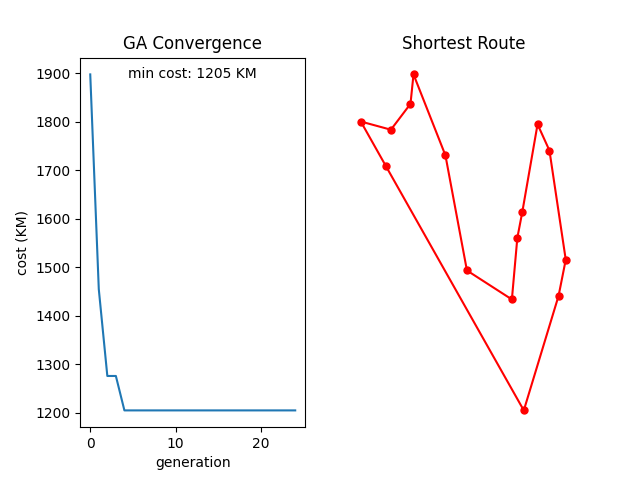
\includegraphics[width=0.4\textwidth]{GeneticAlgorithm_v1.png}\hfill
    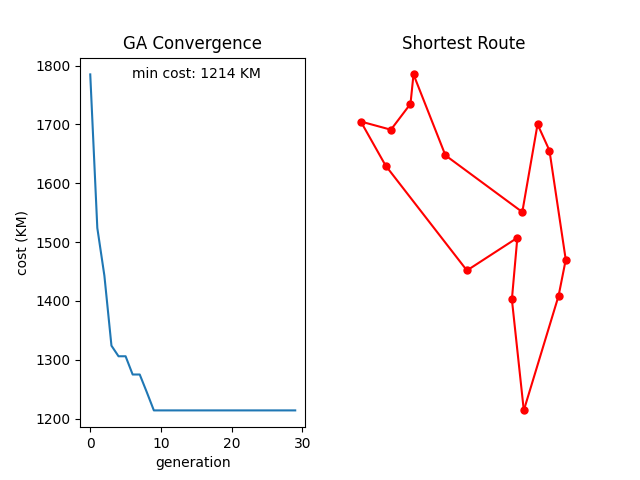
\includegraphics[width=0.4\textwidth]{GeneticAlgorithm_v2.png}\hfill
    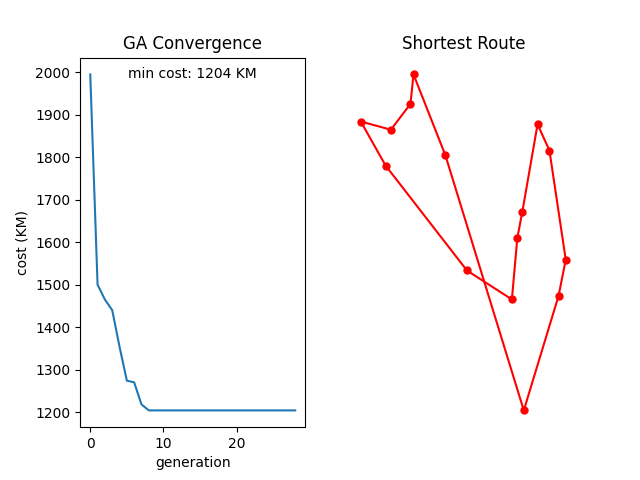
\includegraphics[width=0.4\textwidth]{GeneticAlgorithm_v3.png}\hfill
    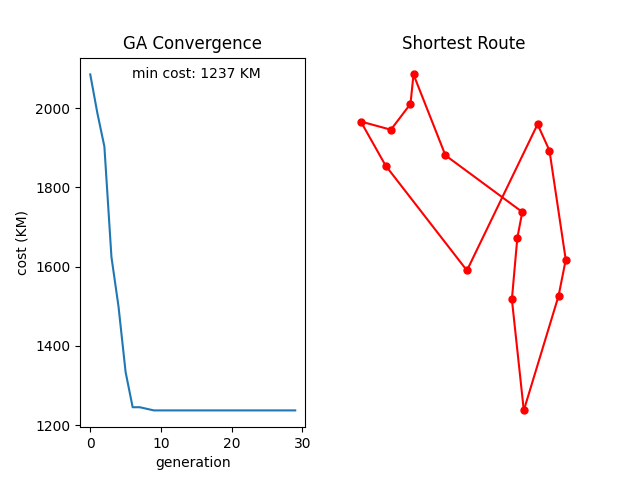
\includegraphics[width=0.4\textwidth]{GeneticAlgorithm_v4.png}\hfill
    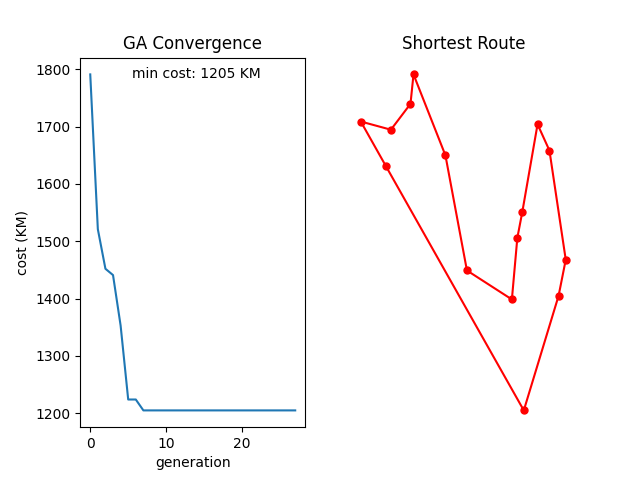
\includegraphics[width=0.4\textwidth]{GeneticAlgorithm_v5.png}
    \caption{Visual of Generations and Shortest Path by GA (15 cities)}
    \label{fig:my_label}
\end{figure}


\section{Analysis}
Based on our experimental tests and simulations, we can distinctly observe the critical differences between simulated annealing and ant colony optimization constructed from our current parameters. SA was considerable faster than ACO in terms of execution time as it was approximately 10.01 times after in n = 15 cities case, and an astonishing 14.09 times faster when n = 50 cities. We also identify that the transformation from 15 cities to 50 had no palpable effect on SA. However, ACO's execution time did increase to a slight extent. Nonetheless, disregarding the execution times for a second, ACO was intelligibly able to find a shorter path than SA consistently. Although the disparity in the 15 cities study was slight, we see the significant difference with the addition of 35 more coordinate points. 
\par Taking a closer inspection on the visualization of the cities and how each of the algorithms determined their optimal shortest path, we see a perceptible difference between the two, particularly in the n = 50 cities case. The ACO algorithm primarily found the closer to optimal solution taking the perimeter path around the city. This is most likely due to the high pheromone concentration aspect of the approach as once the simulated ants determined the shortest distances between cities, they began to prefer that route. However, in the SA visuals, we notice that the increased amount of path intersections and wasted distance due to the initial exploration and quick execution time. Regarding the analysis of the Genetic Algorithm data, given that we utilized a different data set, we will examine this individually. With the current parameters, we saw the variability with the number of generations as it ranged from 24 to 29. However, the execution time of all evolutions as well as the minimum traveling cost remained fairly consistent throughout the tests. The shortest route visuals also followed a perimeter path around the 15 cities similarly to ACO, and the convergence of all trials was approximately 10 generations. 
\par Thus, we can conclude that ACO can be considered the most suitable algorithm if we are optimizing for the shortest distance between the n cities at the cost of a high execution time. The SA algorithm would be appropriate if we are looking for a tremendously fast algorithm with low runtime complexity, but this would come with the trade-off of getting a less than optimal distance. We can presume that GA would be second in order in both the execution time and shortest distance if it was handling the same TSP data set, so this likely won't be considered for an optimal algorithm by researchers in any aspect. We additionally do have to acknowledge that all of these algorithms may possibly give varying results due to perhaps the machine it is running on, or the different parameters and attribute values such as: alpha, beta, initial temperature, cooling rate, etc.

\section{Conclusion and Future Work}
In this paper, we extensively studied some modern approaches to the conventional traveling salesman problem. We additionally presented a qualified study between several optimization techniques including: simulated annealing, ant colony optimization, and genetic algorithm. Each of these algorithms provided a contrasting aspects of randomness and probabilistic measures that would bring limitations to the other algorithms. We concluded that ACO is the most suitable if we are optimizing for the shortest distance, and SA if we were examining pure execution time and complexity. This comparative study brings up an intriguing algorithm that could be tested in the future: a modified approach that incorporates both simulated annealing and the ant colony optimization. With ACO providing the best optimal shortest distance of the three and SA's low execution time, it would be compelling to see whether the algorithms complement each other well or impose their limitations on one another. In terms of future work in this field, there are several fascinating applications of TSP. For instance, the Hyperloop concept that was proposed by Robert Goddard in 1904 which is essentially a vactrain for passengers and freight transportation that would travel underground free of air resistance and friction. In order to design the routes of the vactrain efficiently, we would need to prospectively run algorithms on TSP to determine how it would travel around the United States city to city. At the core of machine learning and artificial intelligence lie the notion of optimization problems. As science and machines continue to advance in their fields, we hope to see the traveling salesman problem be solved optimally in the near future.  


 

\newpage
\bibliographystyle{plain}
\raggedright
\bibliography{./finalproj}

\end{document}